\documentclass{article}
\usepackage[left=0.85in, right=0.85in, top=0.5in, bottom=0.95in]{geometry}
\usepackage[T1]{fontenc}
\usepackage[utf8]{inputenc}
\usepackage[italian]{babel}
\usepackage{graphicx}
\usepackage{wrapfig2}
\usepackage{amsmath}
\usepackage{amssymb}
\usepackage{cases}
\usepackage{gensymb} %simboli come ° = \degree  etc etc
\usepackage{subcaption}
\usepackage{hyperref}
\hypersetup{
	colorlinks=true,
	linkcolor=blue,    
	urlcolor=blue,
	pdfpagemode=FullScreen,
}
\urlstyle{same}
\usepackage{changepage}
\usepackage{lastpage, epstopdf}
\usepackage{fancyhdr}
\usepackage{tcolorbox}
\usepackage{background}
\usepackage{tikz}
\usetikzlibrary{patterns}


%=======HEADER & FOOTER=======%
\def\lesson{Lezione N. 4}
\def\outcome{\textbf{Learning Outcomes:} Outcomes go here. }

\pagestyle{fancy}
\fancyhf{}
\renewcommand{\headrulewidth}{0pt}
\renewcommand{\footrulewidth}{1.4pt}
\lfoot{A.M. $\diamond$ \the\year}
\cfoot{Page \thepage}
\rfoot{\lesson}

%=======CORNELL STYLE FORMAT=======%
\SetBgScale{1}
\SetBgAngle{0}
\SetBgColor{black}
\SetBgContents{\rule{1pt}{0.85\paperheight}}
\SetBgHshift{-1.6in}
\SetBgVshift{-0.1in}

%=======CUSTOM BOXES=======%

\parindent 0ex

%=======BODY=======%
\begin{document}
	\setcounterpageref{secnumdepth}{0}
	\section*{Parte 4} %Date: \hrulefill}
%	\begin{tcolorbox}{\outcome}\end{tcolorbox}

\begin{adjustwidth}{2in}{} 
	
\textbf{{\Large De Saint Venant: Flessione Deviata}} \mbox{} \newline
		Si consideri ora l’azione di un momento $ M $ che giace sul piano di
		sezione $ xy $ applicato sulla faccia finale della trave. Si consideri
		il sistema di riferimento $ xyz $ sempre principale di inerzia e baricentrico. Ora il momento è generico e non più coincidente con quello in $x$ o in $y$. 
		
		Si individuano gli assi $m$ asse dei momenti, perpendicolare per definizione all'asse delle sollecitazione $s$, questo è la traccia sulla sezione del piano dove avviene la la rotazione deviata a causa del momento, contiene il piano di rotazione imposto da $M$. \newline 
		
		Una flessione deviata si può studiare attraverso la composizione di flessioni rette applicate secondo gli assi principali di inerzia.
		
\begin{figure}[H]
	\centering
	\label{fig:screenshot001}
	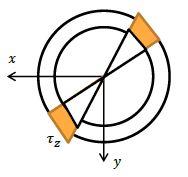
\includegraphics[width=0.5\linewidth]{immagini/screenshot001}
\end{figure}

		In questo modo la sollecitazione è null'altro he una composizione di contributi: 
		\begin{equation} \label{eq:1}
			\sigma_z = \dfrac{M_x}{I_x}y - \dfrac{M_y}{I_y}x
		\end{equation}
		Con segni in accordo al senso di rotazione (antiorario od orario) imposto dal momento. \newline 
		
		Per definizione la traccia sulla sezione del piano neutro è l'asse neutro e si trova attraverso lo studio dei punti non sollecitati:
		\[ \begin{aligned}
			\sigma_z &= 0 \\
			\dfrac{M_x}{I_x}y &- \dfrac{M_y}{I_y}x =0
		\end{aligned} \]
				
\begin{figure}[H]
	\centering
	\label{fig:screenshot002}
	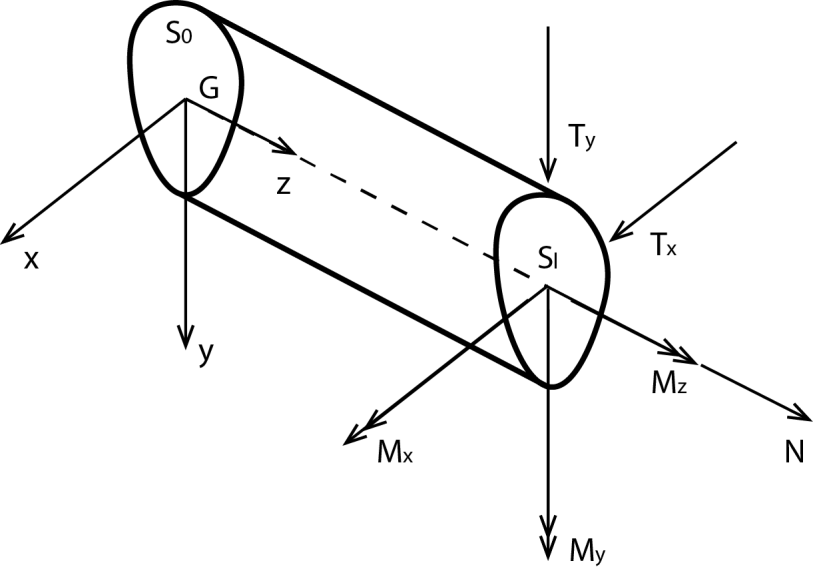
\includegraphics[width=0.5\linewidth]{immagini/screenshot002}
\end{figure}
		
		Si identificano gli angoli $\gamma$, formato dall'asse dei momenti $m$ e dall'asse $x$, e $\beta$ formato dall'asse neutro $n$ e dall'asse $x$.
		\[\dfrac{M_x}{I_x}y - \dfrac{M_y}{I_y}x = 0 \hspace{1cm} \begin{cases}
			M_x = M\cos\gamma \\
			M_y = M\sin\gamma
		\end{cases}\]
		\[\dfrac{ M\cos\gamma}{I_x}y - \dfrac{M\sin\gamma}{I_y}x =0 \Leftrightarrow y = \tan\gamma \dfrac{I_x}{I_y}x\]
		Se, come in questo caso, l'equazione dell'asse neutro non ha il termine noto, passa per l'origine, se il nostro origine è il baricentro, allora l'asse sarà baricentrico.\newline 
		
		L'asse neutro è baricentrico e la sua inclinazione è funzione di $\gamma, I_x, I_y$, ovvero della direzione di applicazione del momento a dalle specifiche caratteristiche della sezione, queste indipendenti dall'entità del momento applicato, in più $M$, l-intensità del momento flettente, non compare: l'asse neutro, oltre che essere baricentrico, è indipendente dal momento applicato. \newline
		Se:
		\[ \tan\beta = \tan\gamma \dfrac{I_x}{I_y} \]
		\[ y = x\tan\beta \]
		
		Si distinguano due casistiche:
		\begin{itemize}
			\item[$ I. $] Se $I_y = I_y \Rightarrow \tan\gamma = \tan\beta $ e l'asse neutro coincide con l'asse dei momenti, ci troviamo nel caso di flessione retta ruotata per sezioni circolari o sezioni caratterizzate da doppio asse di simmetria con distribuzione identica. L’uguaglianza tra
			le inerzie significa che ogni
			riferimento è centrale di inerzia.
			
			\item[$ II. $] Se $I_y \neq I_y \Rightarrow \tan\gamma \neq \tan\beta $ e l'asse neutro NON coincide più con l'asse dei momenti, ci troviamo nel caso di flessione deviata e l'asse delle sollecitazioni non è più ortogonale all'asse neutro ma è inclinato di un angolo $\gamma$.
		\end{itemize}
		 
		
		Perché tutta questa importanza è legata agli assi? Perché sono le tracce dei rispettivi piano. \newline 
		
		Se $\alpha$ identifica l'angolo tra l'asse delle sollecitazioni $s$ e l'asse $x$:
		\[ \alpha = \dfrac{\pi}{2} + \gamma\]
		E l'asse delle sollecitazioni $s$ può essere messo finalmente in relazione con l'asse neutro $n$: 
		\[ \tan\alpha = -\cot\gamma \Rightarrow \tan\gamma = - \dfrac{1}{\tan\alpha}\]
		Poi, ricordando che: 
		\[ \tan\beta = \tan\gamma \dfrac{I_x}{I_y} = - \dfrac{1}{\tan\alpha} \dfrac{I_x}{I_y}\]
		Si giunge infine:
		\[ \tan\beta\tan\alpha = -\dfrac{I_x}{I_y} \]
		
		Dalla definizione è noto che punti alla stessa tensione sono equidistanti dall'asse neutro, tali punti possono essere trovati tracciando le rette parallele a tale asse, in questo modo è possibile tracciare il diagramma delle tensioni su una fondamentale parallela ad $s$ visualizzando una tensione che varia linearmente con la distanza obliqua dal punto generico dall'asse neutro. 
		
		Se con il (') indichiamo grandezze e misure secondo la direzione obliqua, ciò che visualizzeremo sarà: 
		\[ \sigma_z = k \cdot d'_nP\]
		Poiché le distanze devono essere presse rispetto ad assi tra loro coniugati, si dimostri che $s$ ed $n$ lo siano.

\begin{figure}[H]
	\centering
	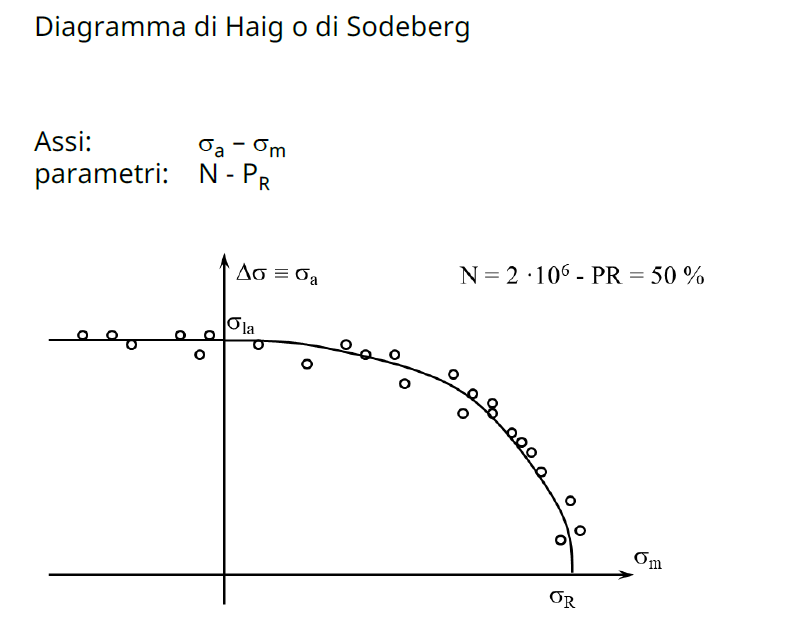
\includegraphics[width=0.5\linewidth]{immagini/screenshot003}
	\label{fig:screenshot003}
\end{figure}		
		
		È più che noto che avendo applicato solo un momento, l'equilibrio a traslazione in direzione $z$ deve risultare nullo:
		\[ N = \int_A\sigma_zdA = k\int_A(d'_nP)dA= kS'_n = 0\]
		Dove con $S'_n$ si è identificato il momento statico espresso in misure oblique. 
		
		Essendo verificato per ipotesi l'equilibrio a traslazione, sarà proprio questo momento statico "obliquo" ad essere nullo, avvalorando così la dimostrazione che $n$ è un asse baricentrico. \newline 
		
		D'altro canto so che il momento intorno ad $s$ anche lui dev'essere nullo perché: (1) ho applicato un momento intorno ad $m$; (2) $s \perp m$ per definizione. 
		
		L'equilibrio a rotazione diviene quindi: 
		\[ M_s = \int_A\sigma_z(d_sP)dA = 0 \]
		
\begin{figure}[H]
	\centering
	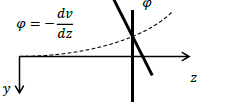
\includegraphics[width=0.5\linewidth]{immagini/screenshot004}
	\label{fig:screenshot004}
\end{figure}

		Scrivendo:
		\[(d_sP) = (d'_sP)\cos\theta\]
		Si giunge a:
		\[ \int_A\sigma_z(d_sP)dA = k\int_A(d'_nP)(d'_sP)\cos\theta dA = k \cdot I'_{ns}\cos\theta\]
		Dove con $I'_{ns}$ si è identificato il momento centrifugo espresso in misure oblique.
		
		Anche qui essendo verificato per ipotesi l'equilibrio a rotazione, sarà proprio questo momento centrifugo "obliquo" ad essere nullo, dimostrando così che gli assi $s$ ed $n$ sono proprio coniugati. \newline 
		
		Applichiamo adesso, infine, l'equilibrio a rotazione intono all'asse $s$, per ipotesi non nullo e uguale al momento deviato imposto: 
		\[M = \int_A\sigma_z(d_mP)dA \]
		
\begin{figure}[H]
	\centering
	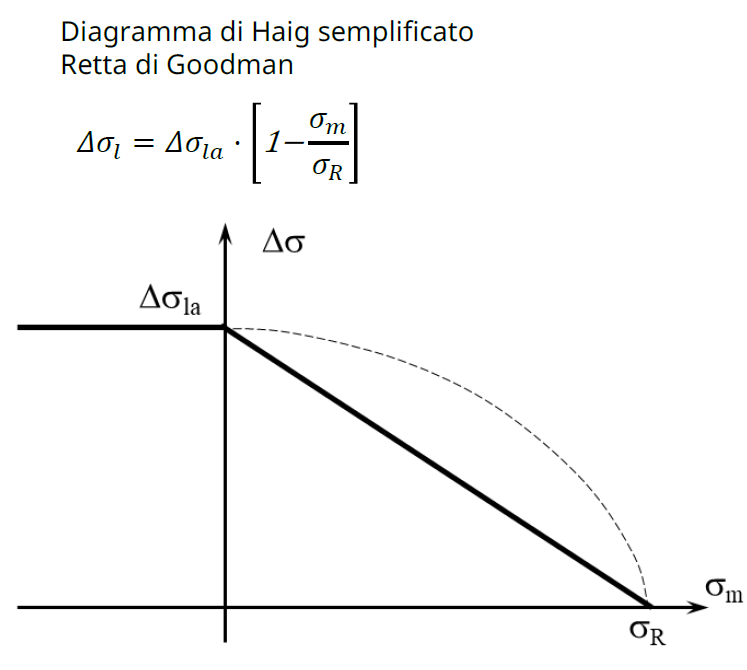
\includegraphics[width=0.4\linewidth]{immagini/screenshot005}
	\label{fig:screenshot005}
\end{figure}

		Scrivendo:
		\[ d_mP = d'_nP + d'_sP\sin\theta\]
		Si giunge a: 
		\[M = \int_Ak(d'_nP)(d'_nP + d'_sP\sin\theta)dA = kI'_n + kI'_{ns}\sin\theta\]
		Poiché poco sopra si è dimostrato che $I'_{ns}=0$:
		\[M=kI'_n \Rightarrow k =\dfrac{M}{I'_n}\]
		
		Si è così infine trovata la funzione che descrive la visualizzazione del momento secondo distanze oblique:
		\[ \sigma_z = \dfrac{M}{I'_n}d'_nP\]
		Tale formula prende il nome di \textbf{Formula Monomia} e può essere manipolata per permettere di tracciare il diagramma delle tensioni su di una fondamentale non più parallela ad $s$ ma ortogonale ad $n$:
		\[ \sigma_z =\dfrac{M}{I'_n}d'_nP \cdot  \dfrac{\cos^2\theta}{\cos^2\theta}= \dfrac{M\cos\theta}{I'_n\cos^2\theta}d'_nP\cos\theta = \dfrac{M_n}{I_n}d_nP\]
		In questo modo non rappresento più il momento in forma obliqua, ma in forma ortogonale rispetto all'asse neutro e la parte di momento di cui terrò conto sarà quella lungo $n$. \newline 
		
		Perché per trovare i valore di momento di flessione non è sufficiente sostituire le coordinate $(x,y$) direttamente in (\ref{eq:1})? La flessione retta era più facilmente visibile e interpretabile, a maggiori $y$ corrispondevano maggiori tensioni; qui no, a meno di sezioni semplici l'andamento del momento non è facilmente leggibile, allora ci si chiede, dov'è la massima tensione? Alla massima distanza dall'asse neutro, scrivendo perciò la relazione monomia si possono trovare i punti più sollecitati e il risultato che ne scaturisce è che questi punti ora li so individuare: una volta trovata l'inclinazione di $n$ traccio due parallele tangenti alla sezione che intersecheranno una fondamentale ortogonale ad $n$. \newline 
		
		Per la linea d'asse le deformazioni risultano essere: 
		\[ \text{Per} ~ M_x \hspace{0.5cm} u = 0 \hspace{0.5cm} v = -\dfrac{1}{2}\dfrac{M_x}{EI_x}z^2 \hspace{0.5cm} w = 0\]
		\[ \text{Per} ~ M_y \hspace{0.5cm} u = \dfrac{1}{2}\dfrac{M_y}{EI_y}z^2 \hspace{0.5cm} v = 0 \hspace{0.5cm} w = 0\]
		\[ \text{Per} ~ M_x +M_y \hspace{0.5cm} u = \dfrac{1}{2}\dfrac{M_y}{EI_y}z^2 \hspace{0.5cm} v = -\dfrac{1}{2}\dfrac{M_x}{EI_x}z^2 \hspace{0.5cm} w = 0\]
		Dove si trova la linea d'asse a seguito di una flessione deviata? Ora l'inflessione è deviata e si trova su di un piano inclinato rispetto ad $x$ ed $y$, in un piano che non è nè $xz$ nè $yz$ ed è individuato dal versore che ha come coseni direttori null'altro che i coefficienti degli spostamenti:
		\[\hat{f} = \left(\dfrac{M_y}{EI_y}; -\dfrac{M_x}{EI_x}\right)\]
		Individua un asse di flessione nel piano di sezione.
		
		Dalla definizione la linea d'asse si inflette secondo un piano ortogonale a quello neutro, che d'altronde ha orientazione data da:
		\[\left( dfrac{M_x}{EI_x};\dfrac{M_y}{EI_y}\right)\]
		E risulta visibilmente ortogonale all'asse di flessione. 
		
		Inoltre si nota che linea d'asse non si allunga e le sezioni rette restano ortogonali all'asse della trave. \newline 
		
		\textbf{{\Large Presso/Tenso - Flessione}} \newline 
		Se si considera l'azione contemporanea di un momento deviato (o di due momenti flettenti retti) e uno sforzo normale, la tensione sarà data dall'equazione:
		\[ \sigma_z = \dfrac{N}{A} + \dfrac{M_x}{I_x}y - \dfrac{M_y}{I_y}x \]
		E l'asse neutro sarà individuato dall'equazione:
		\[ \dfrac{N}{A} + \dfrac{M_x}{I_x}y - \dfrac{M_y}{I_y}x \]
		La sovrapposizione degli effetti può essere sfruttata per definire in questo caso oltre al sistema di forze sopra menzionato, un altro sistema di forze equivalente, un'altra combinazione elastica di momenti e sforzo normale: il caso di un'azione di solo sforzo normale eccentrico applicato in un punto $ C $ detto centro di pressione, diverso dal baricentro, che applica due momenti: 
		\[ M_x = Ne_y \hspace{1cm} M_y = -Ne_x\]
		in questo modo:
		\[ \sigma_z = N\left(\dfrac{1}{A} + \dfrac{e_y}{I_x}y - \dfrac{e_x}{I_y}x\right) \]
\begin{figure}[H]
	\centering
	\label{fig:screenshot006}
	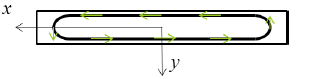
\includegraphics[width=0.2\linewidth]{immagini/screenshot006}
\end{figure}
\newpage		
		\textbf{Ellisse centrale di inerzia} \newline 
		Data una figura $A$ si definisce ellisse centrale di inerzia o ellisse di Culmann del sistema continuo, l'ellisse che ha per centro il baricentro $G$ di $A$ e per semiassi i raggi principali d'inerzia.
		\[ \rho_\xi = \sqrt{\dfrac{I_\xi}{A}} \hspace{1cm} \rho_\eta = \sqrt{\dfrac{I_\eta}{A}} \]
\begin{figure}[H]
	\centering
	\begin{tikzpicture} [>=latex]
	%\draw [thin, help lines] (0,0) grid (5,5);
	\draw (1.5,1) ellipse (2 and 2.5);
	\draw[<->] (1.5,1) -- (3.5,1) node [pos=0.5, below] {$\rho_\xi$};
	\draw[<->] (1.5,1) -- (1.5,3.5) node [pos=0.5, right] {$\rho_\eta$};
\end{tikzpicture}
\end{figure}
	
		Alla massima inerzia corrisponde il semiasse maggiore e viceversa.
		
		L’ellisse
		visualizza sinteticamente le proprietà geometriche della sezione risultando di forma più
		allungata nella direzione di minima inerzia permette di visualizzare dove si sviluppa maggiormente la resistenza inerziale della sezione. \newline 
		
		Un carico applicato equivalente ad una forza applicata in C
		determina delle sollecitazioni che sono date dalla
		sovrapposizione degli effetti:
		\[
		N ~ in ~ C = \begin{cases}
			N \\
			M_x = Ny_C \\
			M_y = -Nx_C
		\end{cases}
		\] 
		E l'asse neutro si può trovare ora in funzione dei raggi d'inerzia: 
		\[ 1+ \dfrac{y_C}{\rho^2_x}y + \dfrac{x_C}{\rho^2_y}x = 0\]
		E diventa una \textit{relazione di coniugio} tra l'asse neutro e quello delle sollecitazioni, tra l'asse neutro e il punto di applicazione $C$ del carico: l'asse neutro si dice retta coniugata rispetto all'ellisse di Culmann del punto $ C $. \newline 
		
		\textit{L'asse neutro è la retta coniugata del punto C nella polarità, avente come conica fondamentale l'ellisse di Culmann della sezione}. \newline 
		
		\textit{Il punto $C$ prende il nome di \textbf{antipolo} e la retta $n$ prende il nome di \textbf{antipolare} del centro $C$ di sollecitazione.} \newline
		
		\textit{Si definisce nocciolo centrale di inerzia (NCI) il luogo degli antipoli delle rette non secanti la sezione
		trasversale della trave.} \newline
		
		\textit{Le rette che rappresentano l'inviluppo convesso della sezione generano la frontiera del nocciolo.}\newline
		
		Allontanandosi dalla retta tangente alla sezione gli antipoli entrano all'interno del NCI. \newline 
		
		Nel caso di sezione rettangolare il NCI corrisponde ad un rombo i cui vertici sono gli antipoli degli assi tangenti i fianchi della sezione, tutti i punti da $A_1$ ad $A_3$ sono gli antipoli delle rette appartenenti al fascio proprio di rette passante per lo spigolo.
		
		Laddove una sezione abbia un fianco rettilineo sarà lì che si avrà un vertice del NCI, laddove ci sarà un vertice della sezione, si avrà invece una linea continua di frontiera del NCI.
		
\begin{figure}[H]
	\centering
	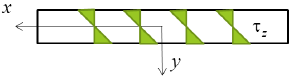
\includegraphics[width=0.7\linewidth]{immagini/screenshot007}
	\label{fig:screenshot007}
\end{figure}

		Si perviene così ad una nuova definizione di frontiera del NCI: 
		
		\hyperref[frontiera]{La frontiera del NCI rappresenta gli antipoli delle rette tangenti.} \newline
		
		È importante il NCI per valutare la pressoflessione. 
		
		La pressofelssione è un elemento cardine nell'ambito civile, è il modo in cui è sollecitata una qualunque colonna (portante): carico verticale + momento o carico verticale eccentrico. 
		
		Ricordi come la flessione deviata generi un asse neutro indipendente dal valore di $M$ ma solo dalla sua inclinazione e dalle caratteristiche della sezione? Ebbene a ciò si aggiunge uno sforzo normale $N/A$, l'asse neutro dipenderà così in questo caso esclusivamente dal punto di applicazione $C$ della forza, perché è antipolare dell'antipolo $C$.
		
		Dato $C$ si può trovare $n$ e viceversa.
		
\begin{figure}[H]
	\centering
	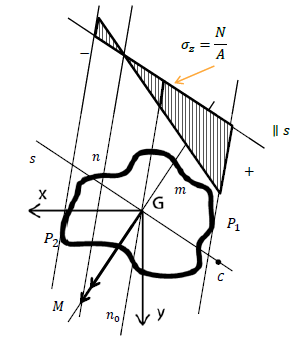
\includegraphics[width=0.5\linewidth]{immagini/screenshot008}
	\label{fig:screenshot008}
\end{figure}

		Si nota infine che il baricentro $G$ si trova sempre in mezzo tra C antipolo ed $n$ antipolare, perché a sua volta l’asse
		neutro si trova sempre, rispetto al baricentro $ G $, dalla parte opposta al centro di
		sollecitazione $ C $; esso si avvicina a $ G $ all’aumentare della distanza di $ C $ da $ G $. \newline 
		
		Se si applica una forza in $A_2$, punto di frontiera del NCI l'asse neutro combacia con $a_2$, un asse neutro tangente implica così l'inesistenza di un andamento a farfalla, la trave in questo modo è sollecitata totalmente a trazione \textbf{O} a compressione, se addirittura si applica una forza all'interno del NCI, l'asse neutro si sposta all'esterno della sezione! Se poi
		il punto di applicazione $ C $ coincide con il baricentro, l’asse neutro esplode all’infinito e ci si riconduce al solo sforzo
		normale. \newline
		
%IMAG nocciolo modificata con diagramma modificato
	
		Tutta la struttura è così caricata da tensioni di un solo segno, che è meglio di un andamento a farfalla soprattutto per materiali non isotropi, che non hanno lo stesso comportamento a trazione o compressione. 
		
		Infatti per una colonna, quello che si fa per far cadere il carico nel all'interno del NCI, è piazzare due architravi equamente caricati così da bilanciare il contributo del carico sovrastante. \newline 
		
		Infine, la linea d'asse della pressoflessione si inflette secondo un piano di sezione che segue le regole della flessione deviata, quindi ortogonalmente al piano neutro, ed in più subisce un allungamento o compressione dovuto allo sforzo normale aggiunto. 
		
		
		
		
	
		
		
		
		
		
		
		
		
		 
		
		
		
	\newpage
	{\Large \textbf{NOTE}}
%	\vfill
%\begin{tcolorbox}[height=4.5cm]
%	This box has a height of 4.5cm.
%\end{tcolorbox}

%DA DECOMMENTARE PER AVERE LA VERSIONE STAMPABILE A DUE PAGINE 	
%	\newpage
%		\null
%		\vfill
%\begin{tcolorbox}[height=4.5cm]
%	This box has a height of 4.5cm.
%\end{tcolorbox}
%		
\end{adjustwidth}
\end{document}